\documentclass[twocolumn,a4j]{jsarticle}
\setlength{\topmargin}{-20.4cm}
\setlength{\oddsidemargin}{-10.4mm}
\setlength{\evensidemargin}{-10.4mm}
\setlength{\textwidth}{18cm}
\setlength{\textheight}{26cm}

\usepackage[top=13truemm,bottom=20truemm,left=15truemm,right=15truemm]{geometry}
\usepackage[latin1]{inputenc}
\usepackage{amsmath}
\usepackage{amsfonts}
\usepackage{amssymb}
\usepackage[dvipdfmx]{graphicx}
\usepackage[dvipdfmx]{color}
\usepackage{listings}
\usepackage{listings,jvlisting}
\usepackage{geometry}
\usepackage{framed}
\usepackage{color}
\usepackage[dvipdfmx]{hyperref}
\usepackage{ascmac}
\usepackage{enumerate}
\usepackage{tabularx}
\usepackage{cancel}
\usepackage{scalefnt}

\renewcommand{\figurename}{Fig.}
\renewcommand{\tablename}{Table }

\lstset{
basicstyle={\ttfamily},
identifierstyle={\small},
commentstyle={\smallitshape},
keywordstyle={\small\bfseries},
ndkeywordstyle={\small},
stringstyle={\small\ttfamily},
frame={tb},
breaklines=true,
columns=[l]{fullflexible},
xrightmargin=0zw,
xleftmargin=3zw,
numberstyle={\scriptsize},
stepnumber=1,
numbersep=1zw,
lineskip=-0.5ex
}

\makeatletter
\def\@maketitle
{
\begin{center}
{\LARGE \@title \par}
\end{center}
\begin{flushright}
{\large \@date}\\
{\large{京都工芸繊維大学 工芸科学部 機械工学課程}}\\
{\large \@author}
\end{flushright}
\par\vskip 1.5em
}
\makeatother

\setcounter{tocdepth}{3}

\author{来代 勝胤 / Masatsugu KITADAI}
\title{令和3年度 12月度 報告書}
\date{2021/12/24}

\begin{document}
\columnseprule=0.1mm

\maketitle
\section*{報告内容}
\begin{enumerate}[1.]
    \item 進捗状況
    \item 模擬実験の実施
    \item データ処理プログラムの作成
    \item プログラムの適用結果
    \item 今月の進捗と今後の予定
\end{enumerate}

\section{進捗状況}
今月は,形状比較実験を行うにあたり,実験データ処理プログラムの作成を行った.
また,その有用性を確かめるために現在の実験装置を用いて模擬実験を行った.

\section{模擬実験の実施とその手順}
今後の実験を行うにあたり,その手順を明確に決定しておく必要がある.
大量のデータを一度にプログラムで処理できるようにするため,
測定手順を以下のように定めた.\\

\begin{figure}[htbp]
    \footnotesize
    \begin{center}
        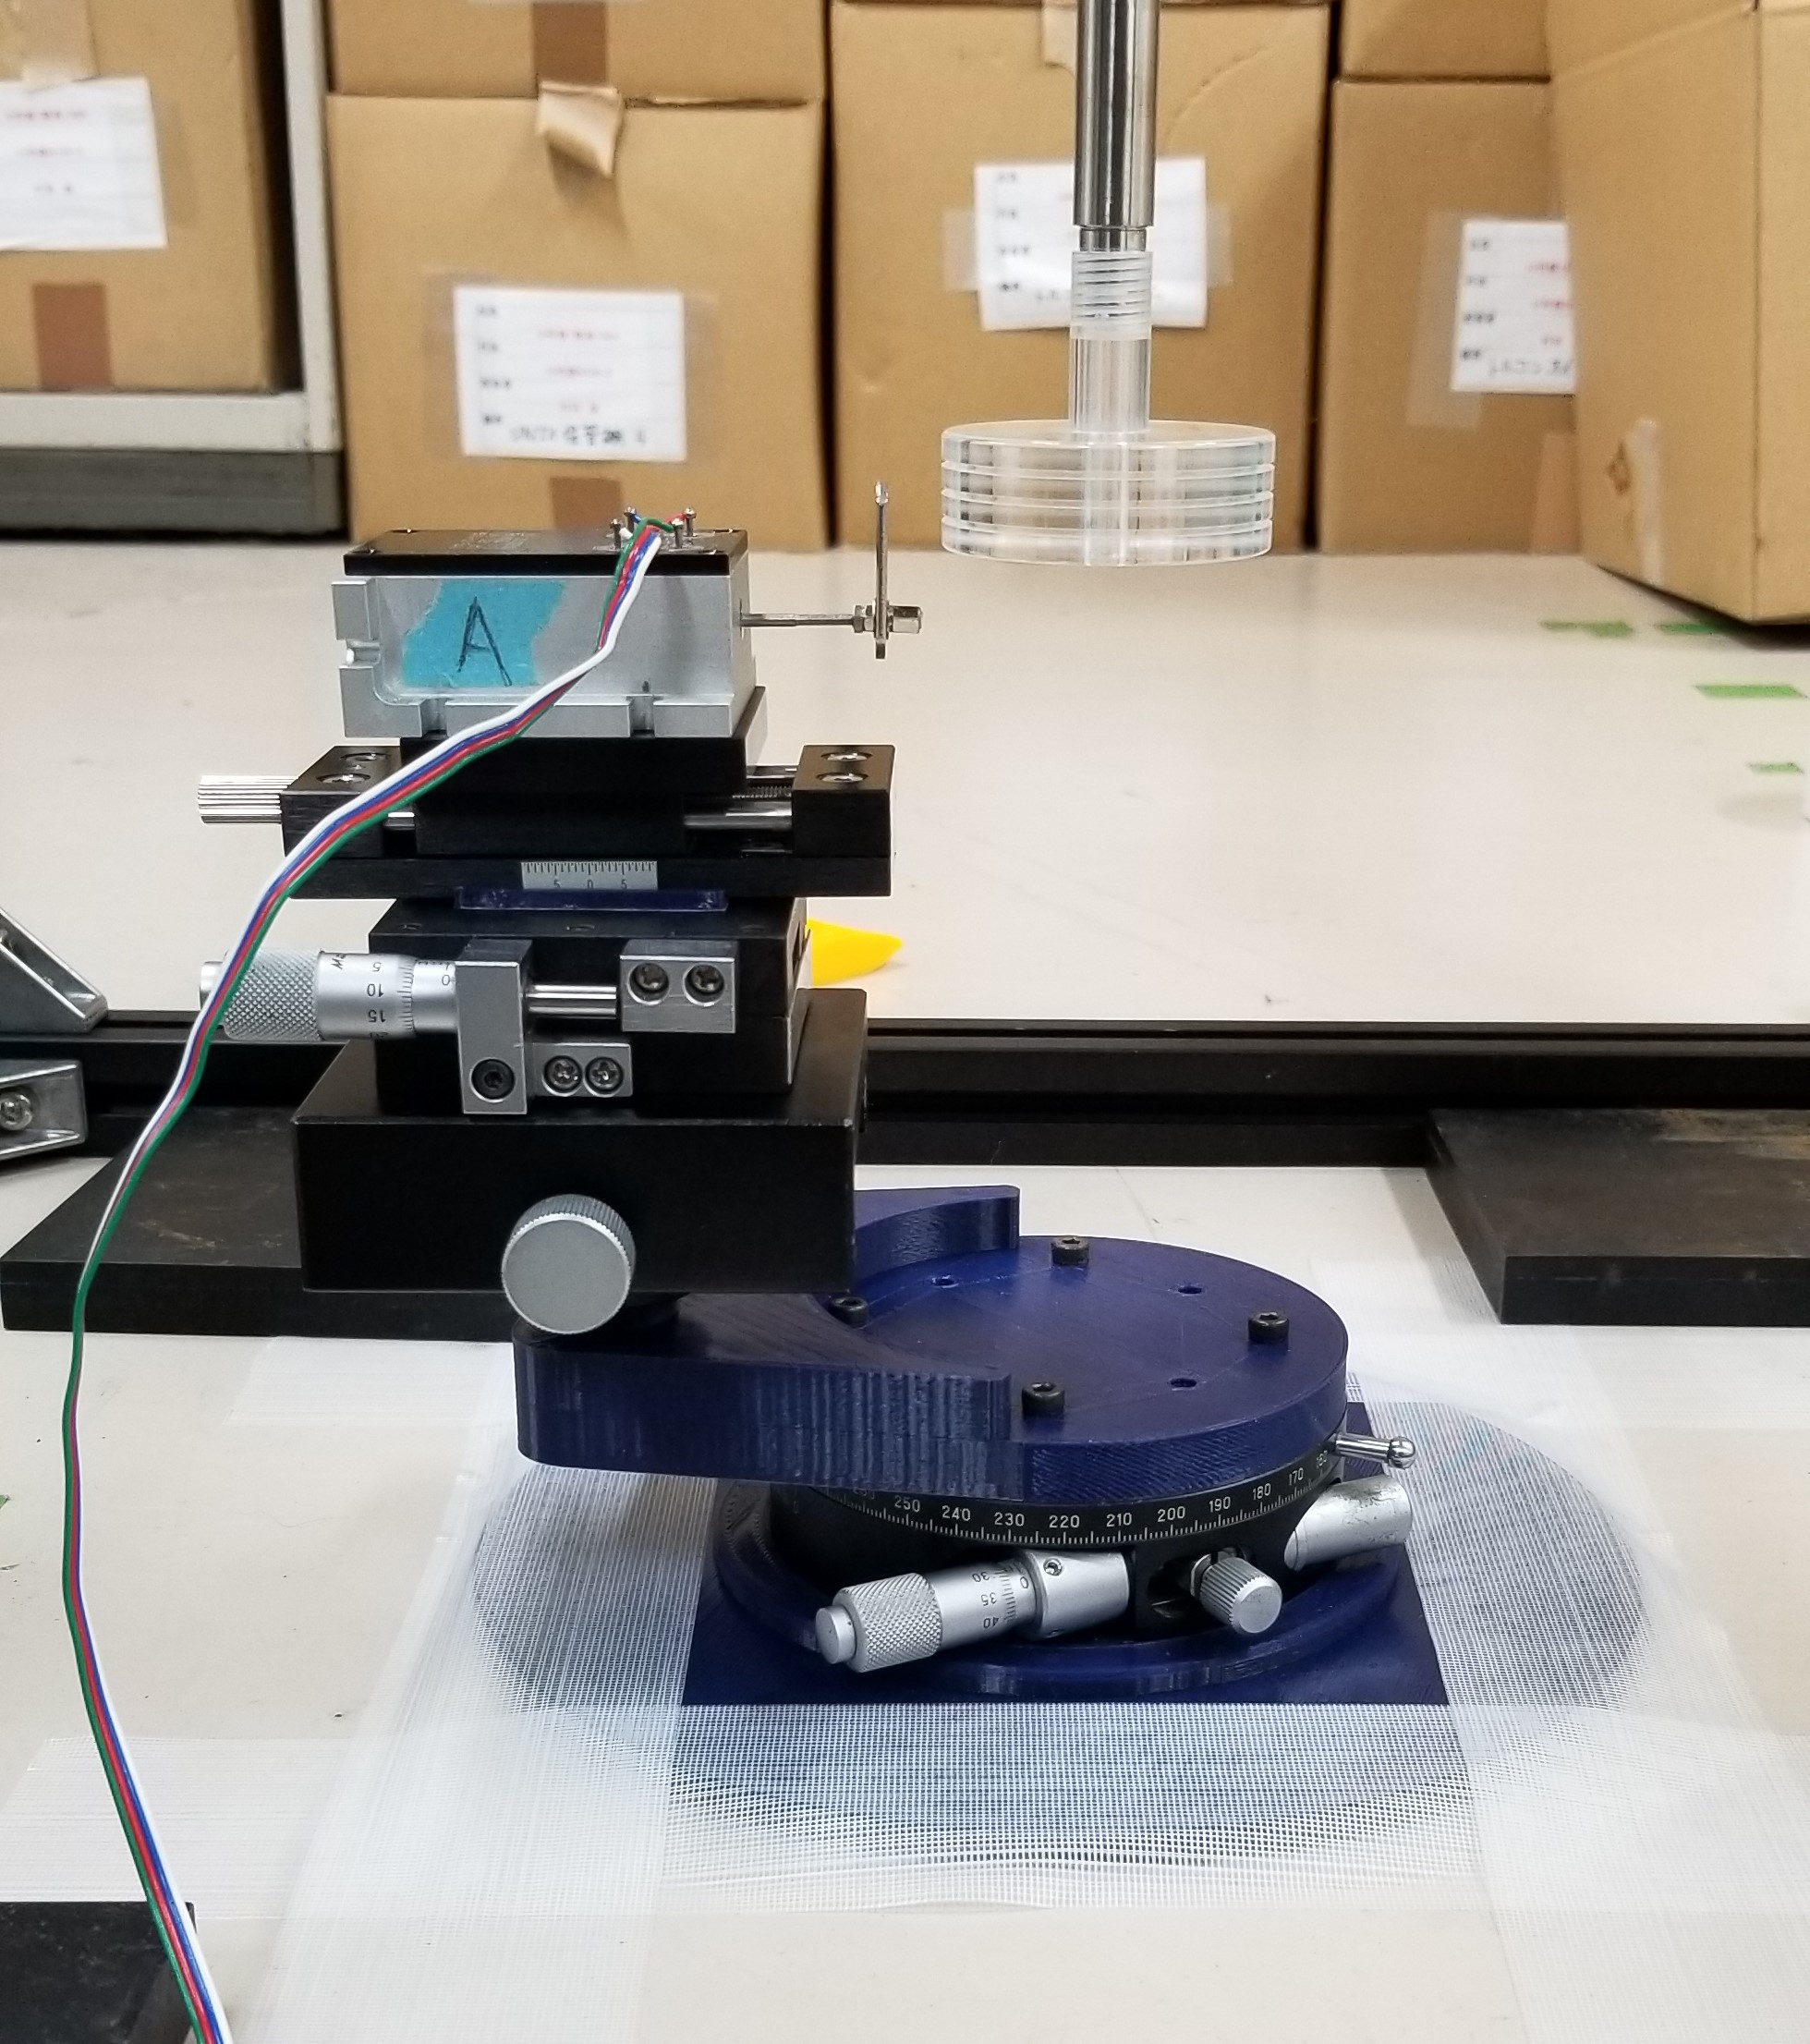
\includegraphics[width=75mm]{../images_3/device_1.jpg}
        \caption{Experimental device}
    \end{center}
\end{figure}

\newpage

\subsection{実験条件}
今回行った模擬実験の条件は以下の図の通りである.
なお,測定角度については,処理プログラムにてFFTを適用する関係上,
2の乗数の値となる16とした.
\begin{table}[htbp]
    \begin{center}
        \begin{tabular}{|p{30mm}|p{20mm}|p{30}|}
            \hline
            \multicolumn{1}{|c|}{\textgt{項目}} & \multicolumn{1}{|c|}{\textgt{条件数}} & \multicolumn{1}{|c|}{\textgt{備考}}\\ \hline
            \multicolumn{1}{|c|}{試験片}                    & \multicolumn{1}{|c|}{1} & \multicolumn{1}{|c|}{\textgt{円筒:現在の実験装置で使用}}  \\ \hline
            \multicolumn{1}{|c|}{測定角度}                    & \multicolumn{1}{|c|}{16} & \multicolumn{1}{|c|}{\textgt{22.5度ごとの測定}}  \\ \hline
            \multicolumn{1}{|c|}{試行回数}                    & \multicolumn{1}{|c|}{1} & \multicolumn{1}{|c|}{\textgt{}}  \\ \hline
        \end{tabular}
    \end{center}
\end{table}

また,今後の実験条件として,以下のように想定している.
\begin{table}[htbp]
    \begin{center}
        \begin{tabular}{|p{30mm}|p{20mm}|p{30}|}
            \hline
            \multicolumn{1}{|c|}{\textgt{項目}} & \multicolumn{1}{|c|}{\textgt{条件数}} & \multicolumn{1}{|c|}{\textgt{備考}}\\ \hline
            \multicolumn{1}{|c|}{試験片}                    & \multicolumn{1}{|c|}{3} & \multicolumn{1}{|c|}{\textgt{円筒・円柱・角柱}}  \\ \hline
            \multicolumn{1}{|c|}{測定角度}                    & \multicolumn{1}{|c|}{32} & \multicolumn{1}{|c|}{\textgt{11.25度ごとの測定}}  \\ \hline
            \multicolumn{1}{|c|}{試行回数}                    & \multicolumn{1}{|c|}{5回程度} & \multicolumn{1}{|c|}{\textgt{検討中}}  \\ \hline
        \end{tabular}
    \end{center}
\end{table}

\subsection{測定条件}
    \begin{itemize}
        \item サンプリング周期は5[Hz]とする
        \item ロードセルをマイクロステージを用いて\\
              0.03 [mm] ずつ移動させ,
              作用力を加え電圧を測定する
        \item 基準を0[mm]として,0.03[mm],0.06[mm],0.09[mm],0.12[mm]の計4回移動させる
    \end{itemize}

\subsection{測定準備}
    \begin{enumerate}[(1)]
        \item ロードセルを測定する角度に固定
        \item 粗動用ダイヤルでロードセルを大まかな位置に設定
        \item マイクロステージを動かしてロードセルが供試体に接触する位置を0.01[mm]単位で特定
        \item その位置を基準に測定を開始する
    \end{enumerate}

\subsection{測定手順}
    \begin{enumerate}[(1)]
        \item 測定開始から30秒間待機する
        \item 40秒間の測定時間
        \item 30秒間のマイクロステージ操作時間
        \item (2),(3)の作業を5回繰り返す (70秒周期)\\
              ※ 5回目はロードセル,供試体を非接触状態にする
    \end{enumerate}

\newpage

\subsection{実験結果}
実施した模擬実験の結果を以下のFig.2,Fig.3に示す.
ここでは例として,0度における結果を示している.

\begin{figure}[htbp]
    \footnotesize
    \begin{center}
        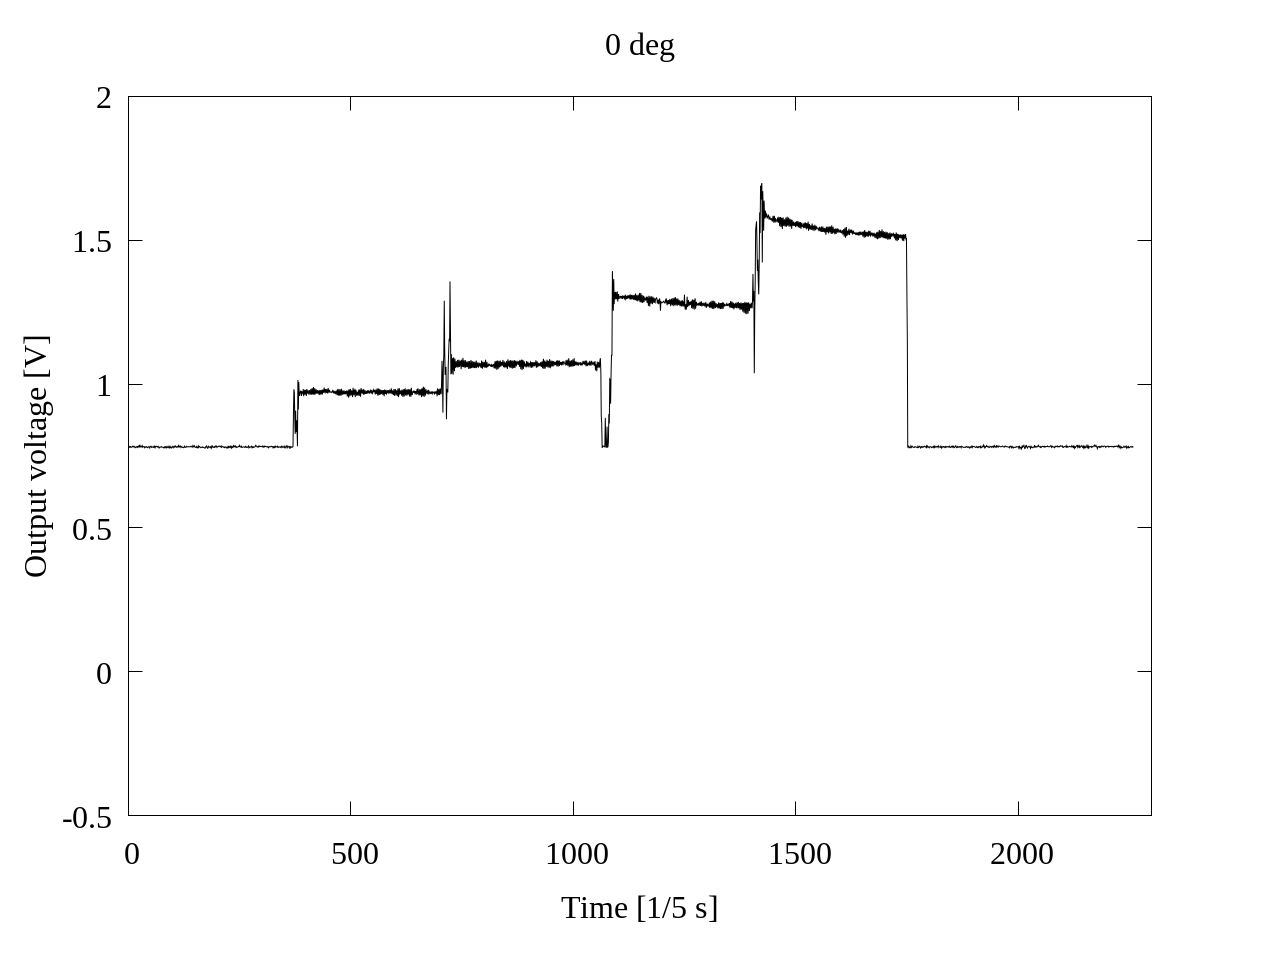
\includegraphics[width=80mm]{../images_2/01-1_loadcell/01_loadcell_0.png}
        \caption{Acting force from 0 [deg] (loadcell)}
        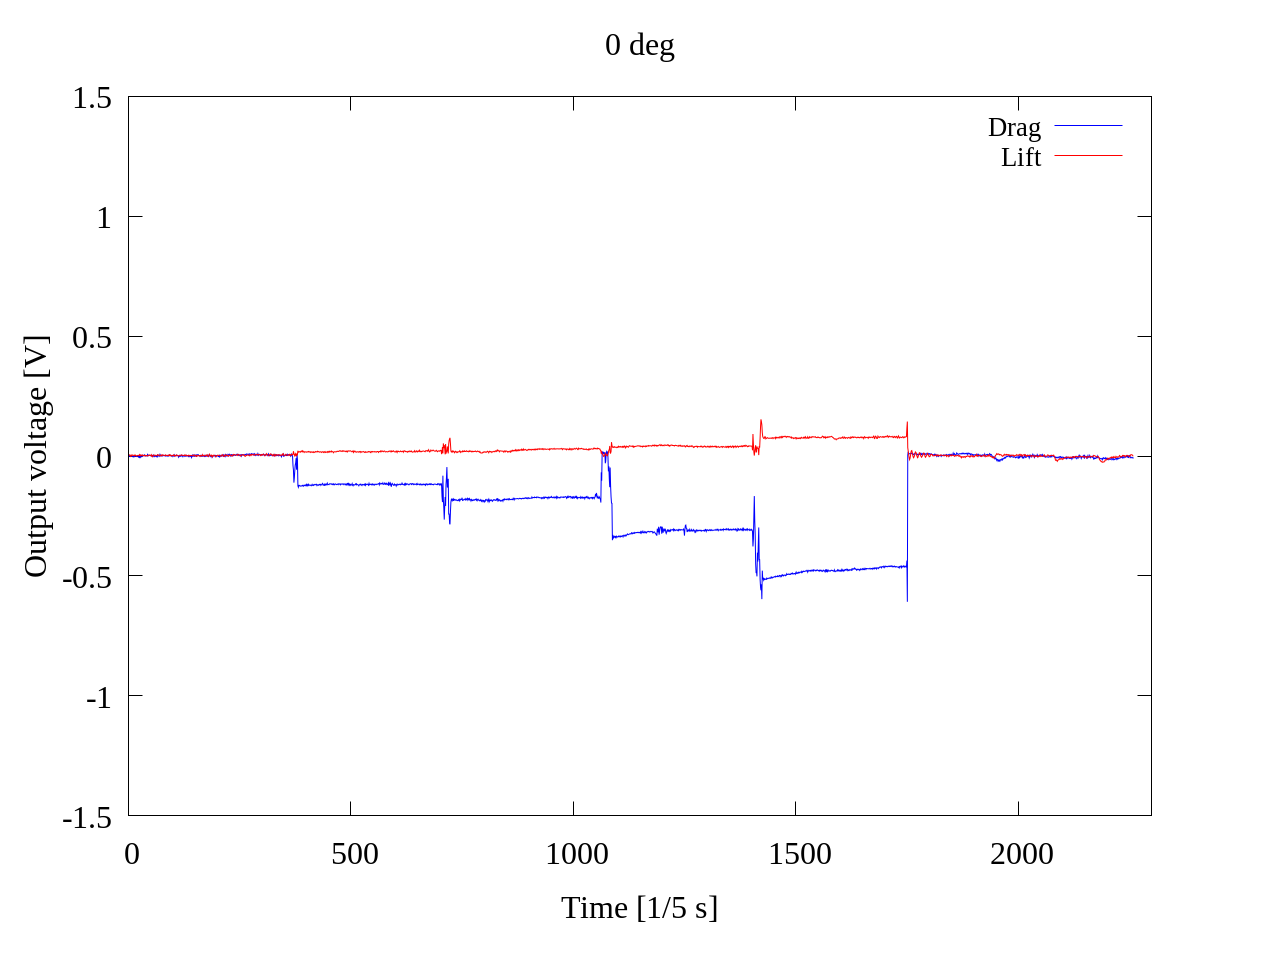
\includegraphics[width=80mm]{../images_2/01-2_strainsensors/01_strainsensors_0.png}
        \caption{Acting force from 0 [deg] (strainsensors)}
    \end{center}
\end{figure}

\section{データ処理プログラムの作成}
実験を一定の手順で行うことにより,
プログラムを複数のデータに一斉に適用することができる.\\

\subsection{データ処理の手順}
実験の目的は,実験装置の出力電圧から作用力へ正しく変換することである.
% その目的を達成するにあたって以下の2項目を達成する必要がある.
この目的を達成するために,以下のような処理手順のプログラムを作成した.
% \begin{enumerate}[(1)]
%     \item 現在使用している実験装置の特徴を理解する
%     \item 実際の作用力と実験装置の出力電圧の対応関係を明らかにする
% \end{enumerate}

% これらを達成するために,以下のような順序でプログラムを作成した

    \begin{enumerate}[(1)]
        \item ドリフト補正
        \item 各距離における平均値の算出
        \item ロードセルとひずみセンサの出力電圧の関係性を\\評価する近似直線を算出
        \item 角度ごとの直線の傾きから理論値を算出
        \item FFTを用いて位相角を算出
        \item 作用力方向と実験装置の設置方向の角度の算出
        \item 抗力及び揚力方向のひずみセンサの取付角の算出
    \end{enumerate}

\newpage

\subsection{ドリフト補正}
以前,作用力測定の結果の解析に用いたアルゴリズムをもとに
ドリフト補正プログラムを作成し,結果に適用した.

\begin{enumerate}[(1)]
    \item 測定開始直後及び終了直前のデータ(30秒/150点)における平均値を算出
    \item 算出した2つの平均値を結び,直線を作成
    \item 元データと直線の差をとり,補正値として採用する
\end{enumerate}

以下のFig.4~Fig.6に0度における適用結果を示す.

\begin{figure}[htbp]
    \footnotesize
    \begin{center}
        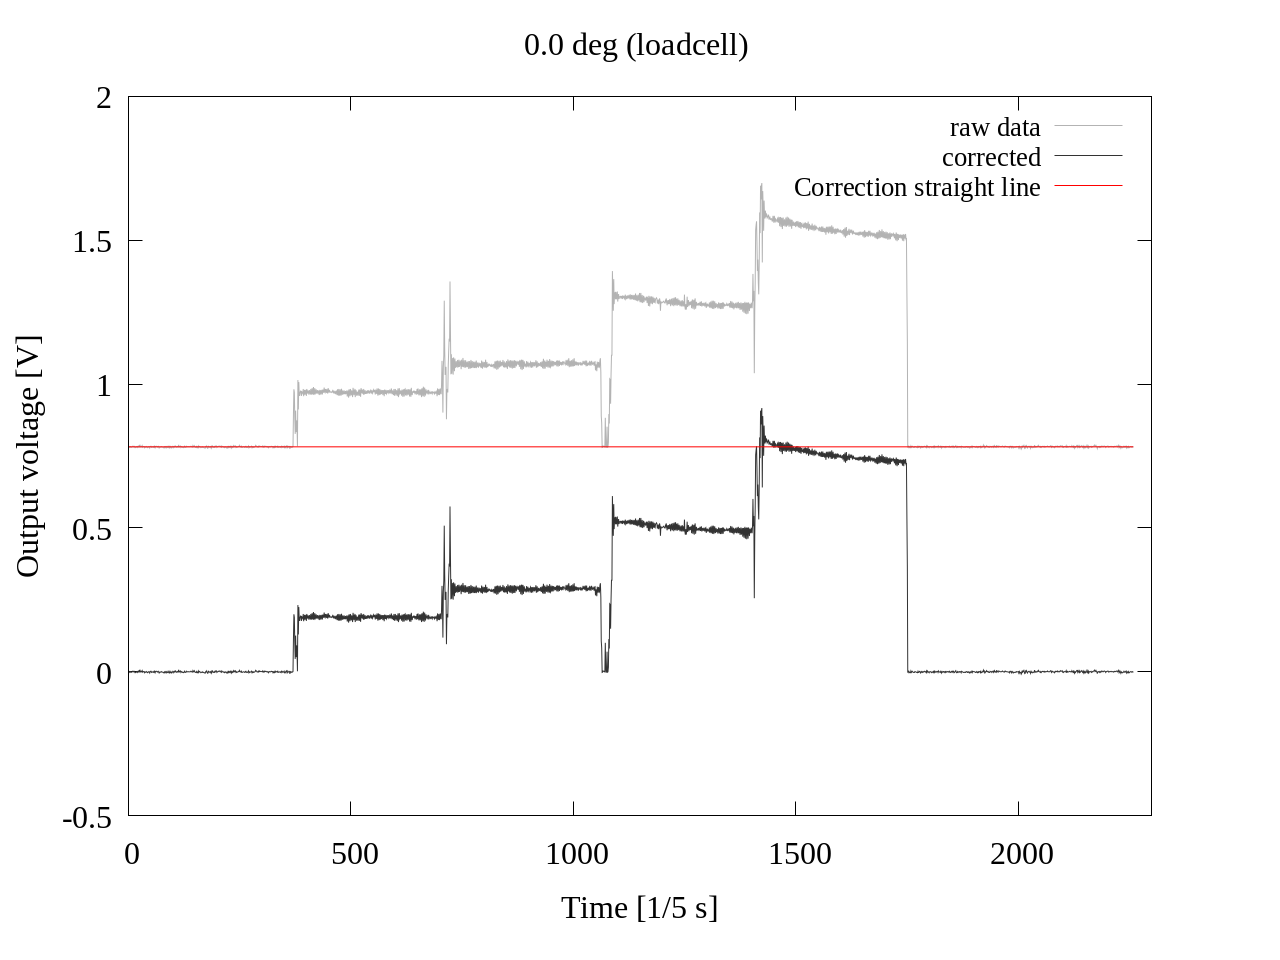
\includegraphics[width=78mm]{../images_2/02-1_loadcell/02_loadcell-drift_0.png}
        \caption{Drift correction 0.0 [deg] (loadcell)}
        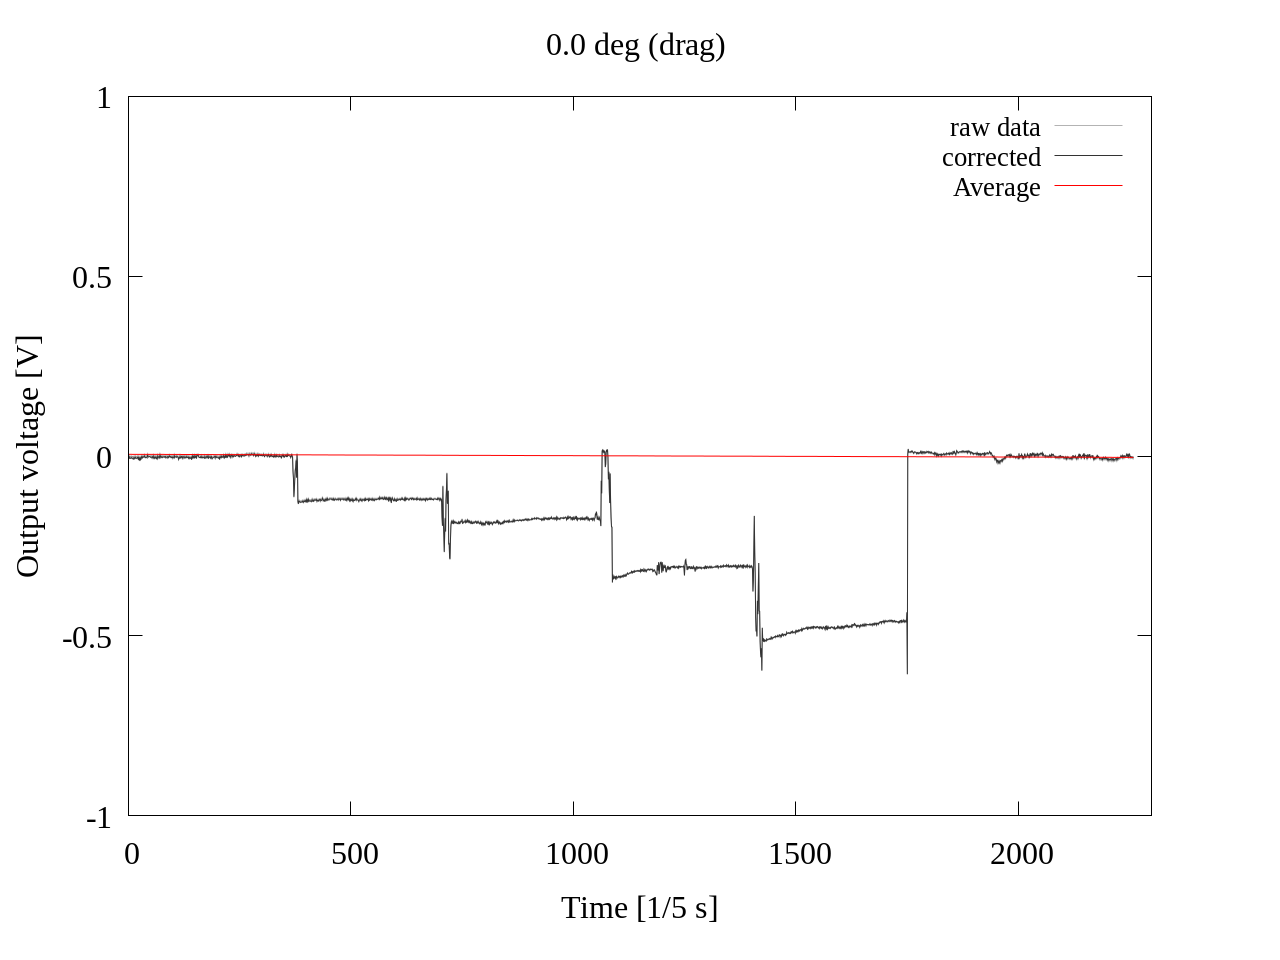
\includegraphics[width=78mm]{../images_2/02-2_drag/02_drag-drift_0.png}
        \caption{Drift correction 0.0 [deg] (drag)}
        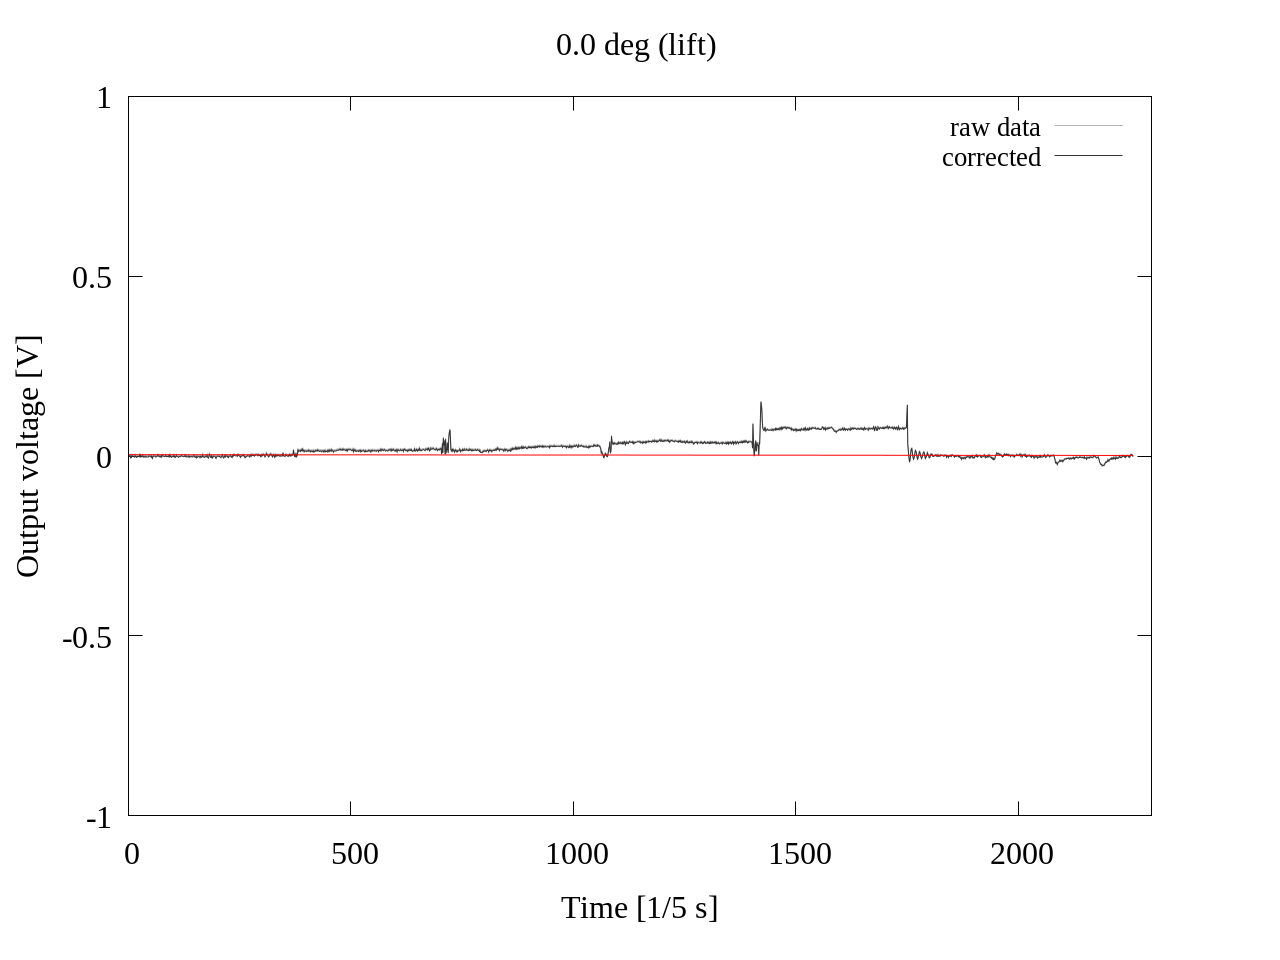
\includegraphics[width=78mm]{../images_2/02-3_lift/02_lift-drift_0.png}
        \caption{Drift correction 0.0 [deg] (lift)}
    \end{center}
\end{figure}

\newpage

\subsection{平均値の算出}
実験手順にしたがって,プログラムの適用範囲を定め
それぞれの距離における出力電圧について平均値を算出した
以下のFig.7~Fig.9に0度における適用結果を示す.

\begin{figure}[htbp]
    \footnotesize
    \begin{center}
        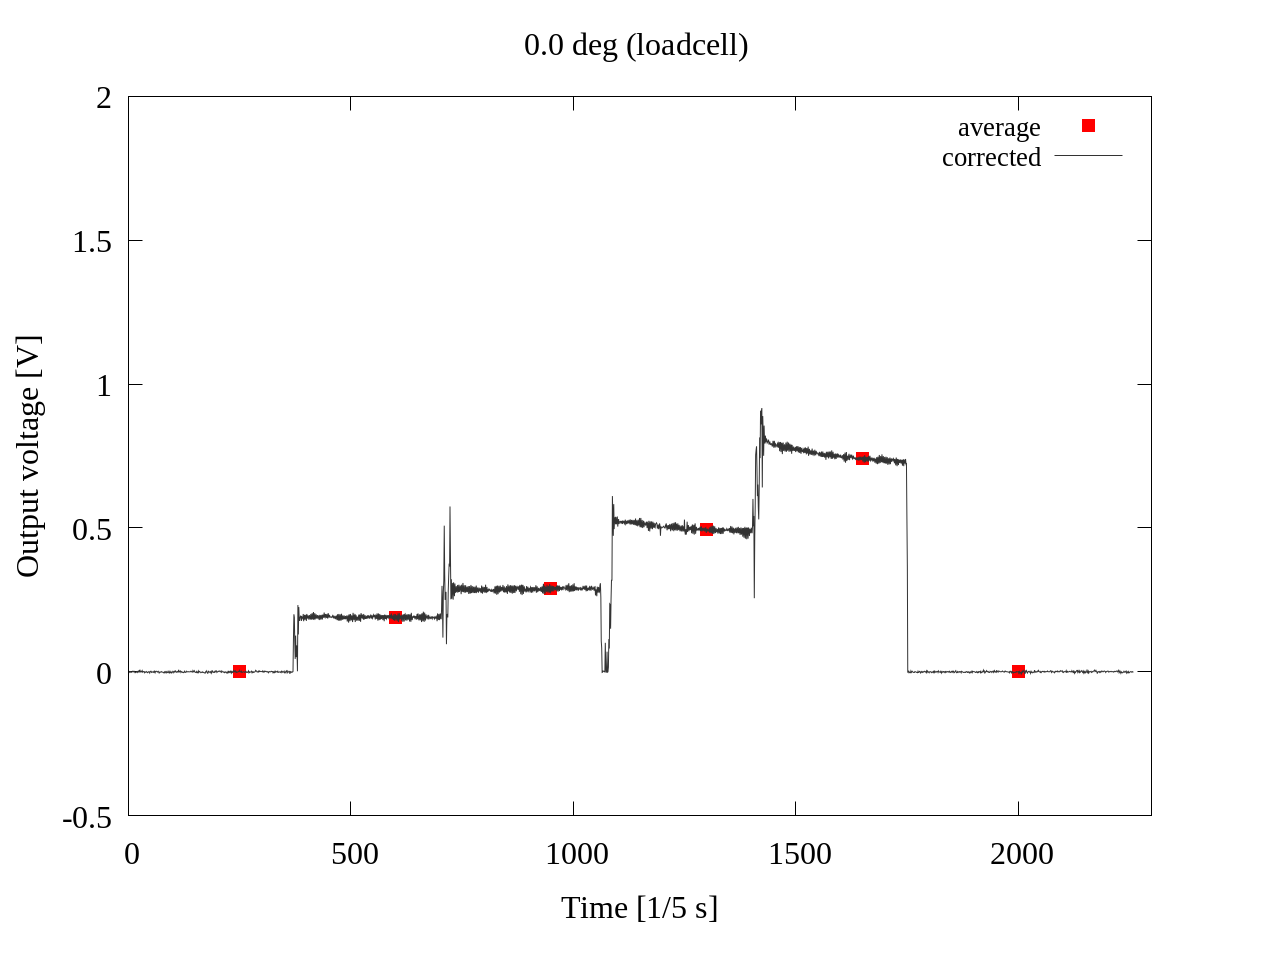
\includegraphics[width=80mm]{../images_2/03-1_loadcell/03_loadcell_average_0.png}
        \caption{Acting force average 0.0 [deg] (loadcell)}
        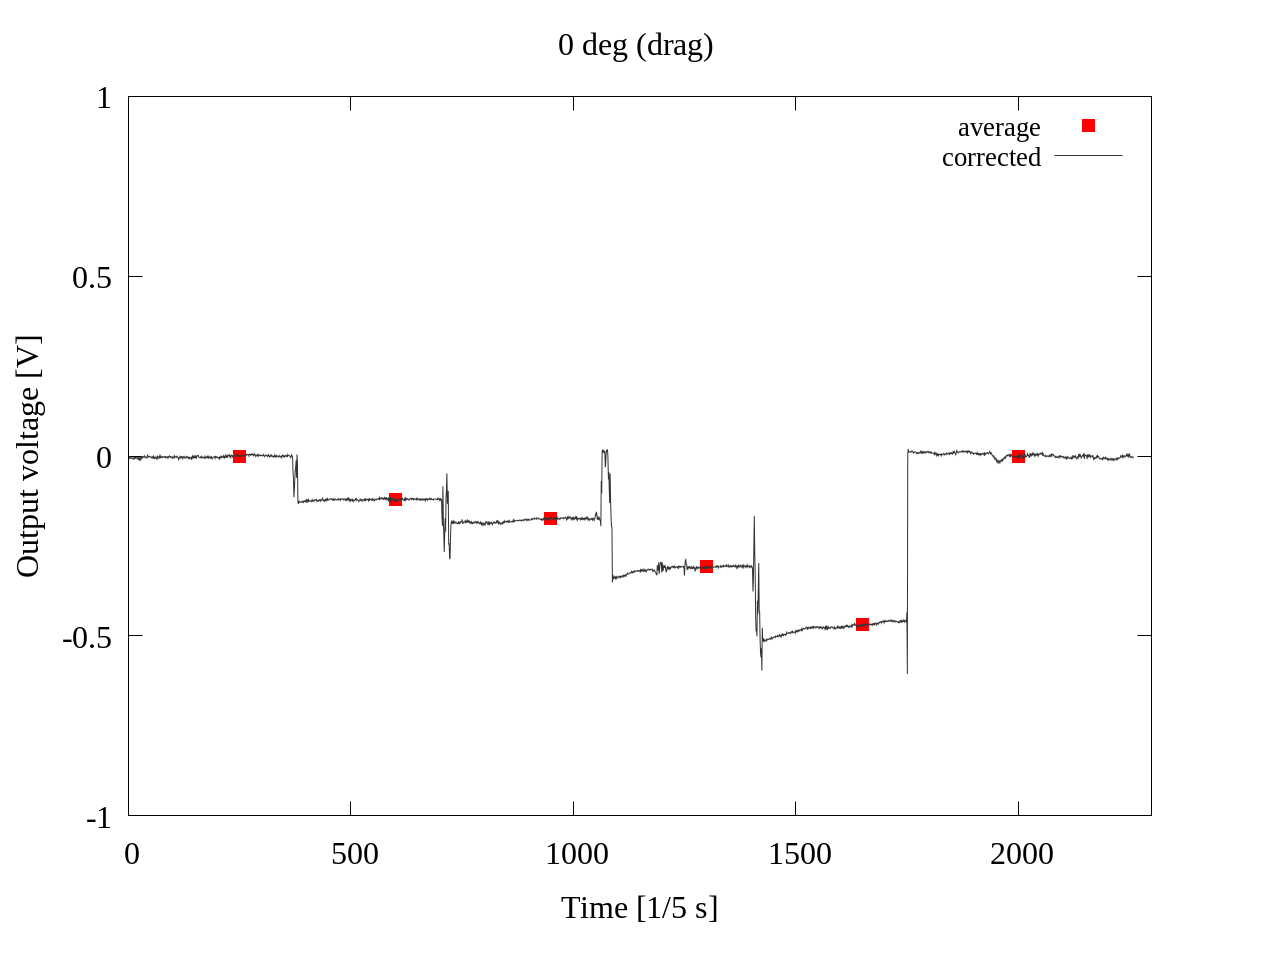
\includegraphics[width=80mm]{../images_2/03-2_drag/03_drag_average_0.png}
        \caption{Acting force average 0.0 [deg] (drag)}
        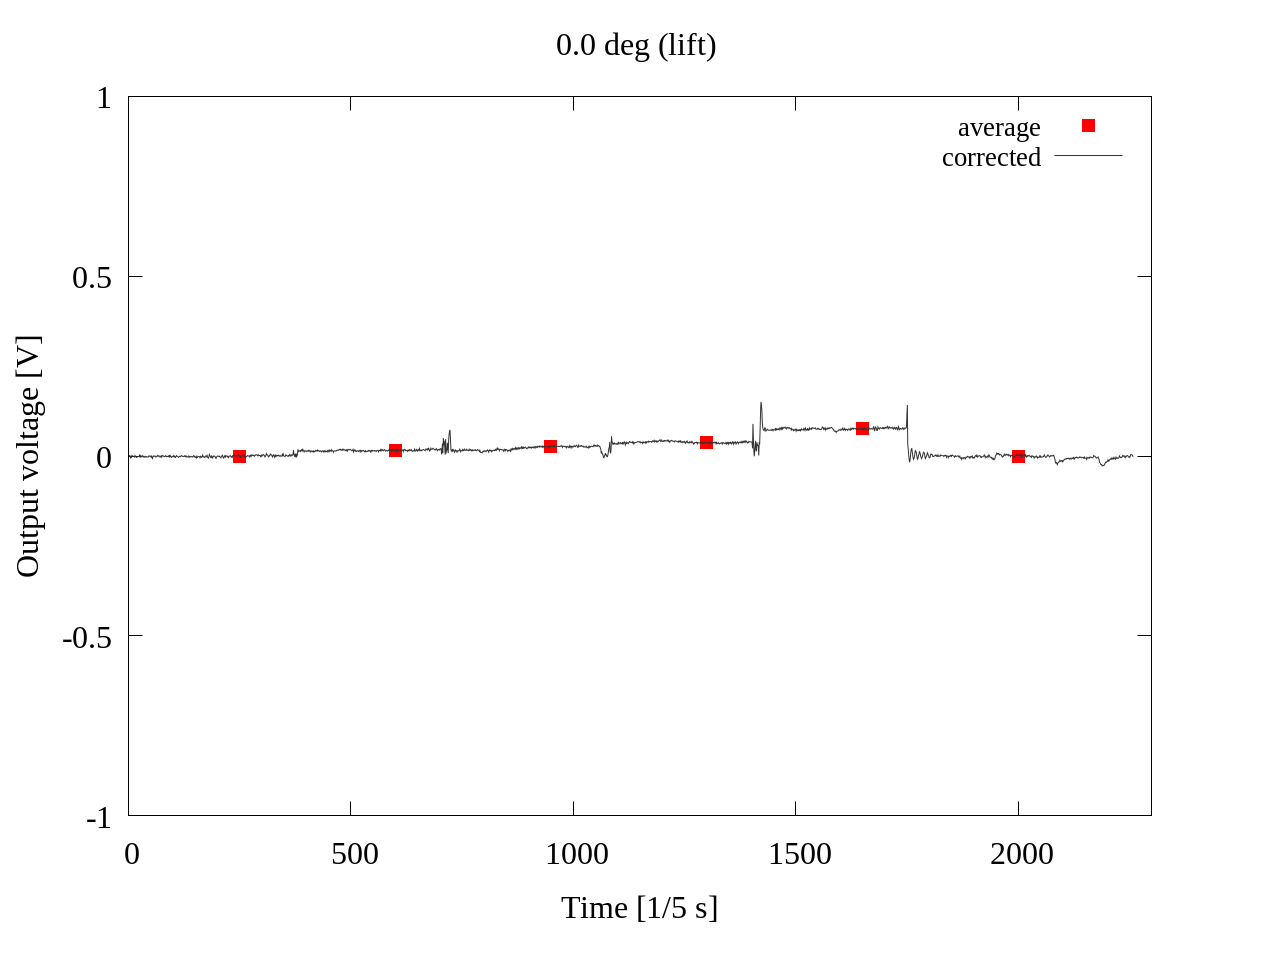
\includegraphics[width=80mm]{../images_2/03-3_lift/03_lift_average_0.png}
        \caption{Acting force average 0.0 [deg] (lift)}
    \end{center}
\end{figure}

\newpage

\subsection{近似直線の算出}
算出した平均値を用いて,ロードセルの出力電圧とひずみセンサの出力電圧についての
関係性を求める.ここでは,それぞれの方向について最小二乗法を用いて近似式を作成した.
以下のFig.10~Fig.12に0度~45度における適用結果を示す.

\begin{figure}[htbp]
    \footnotesize
    \begin{center}
        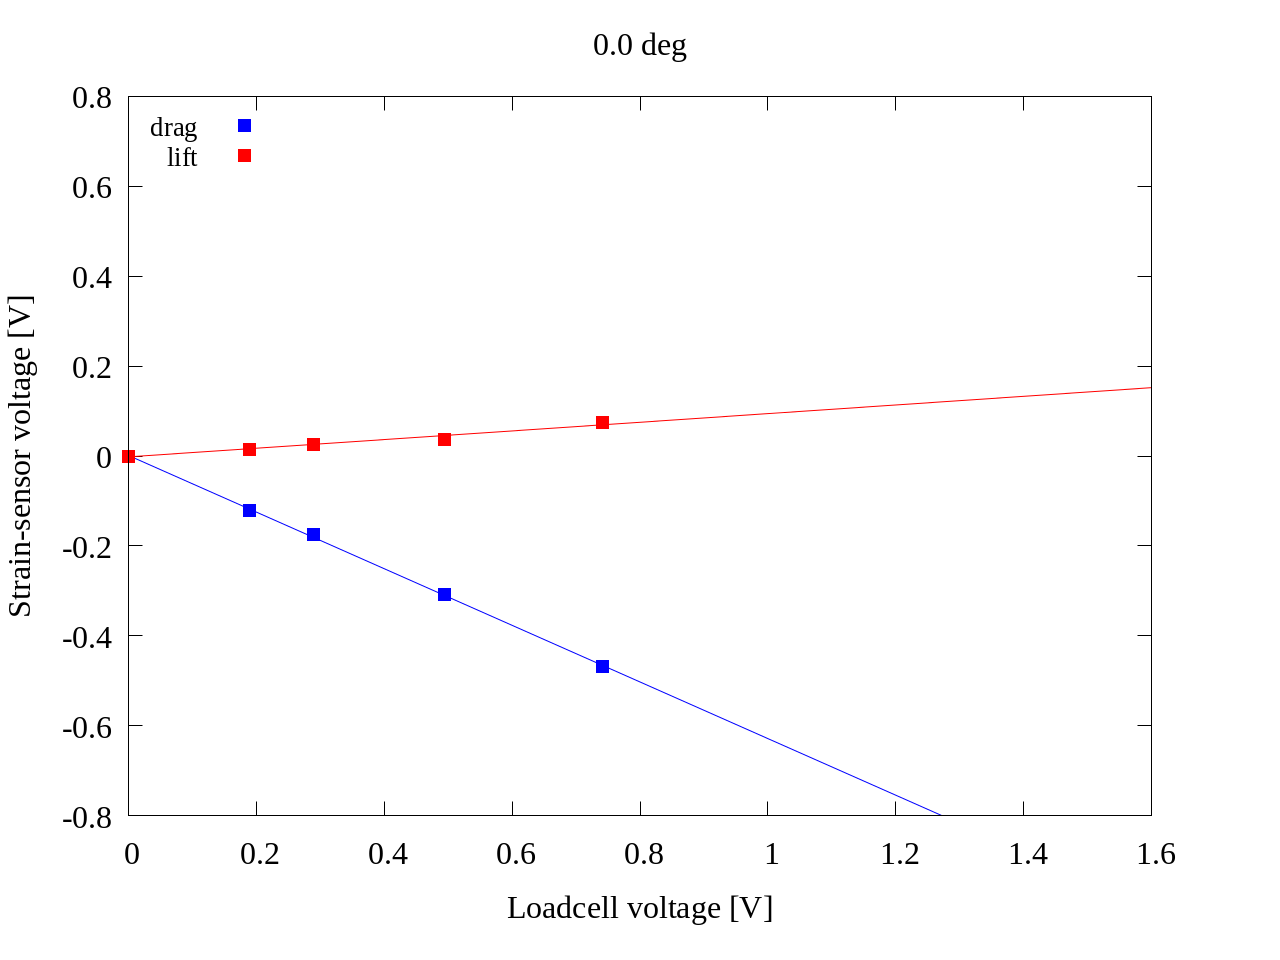
\includegraphics[width=80mm]{../images_2/04/04_linear_0.png}
        \caption{Correlation between loadcell and strainsensors 0.00 [deg]}
        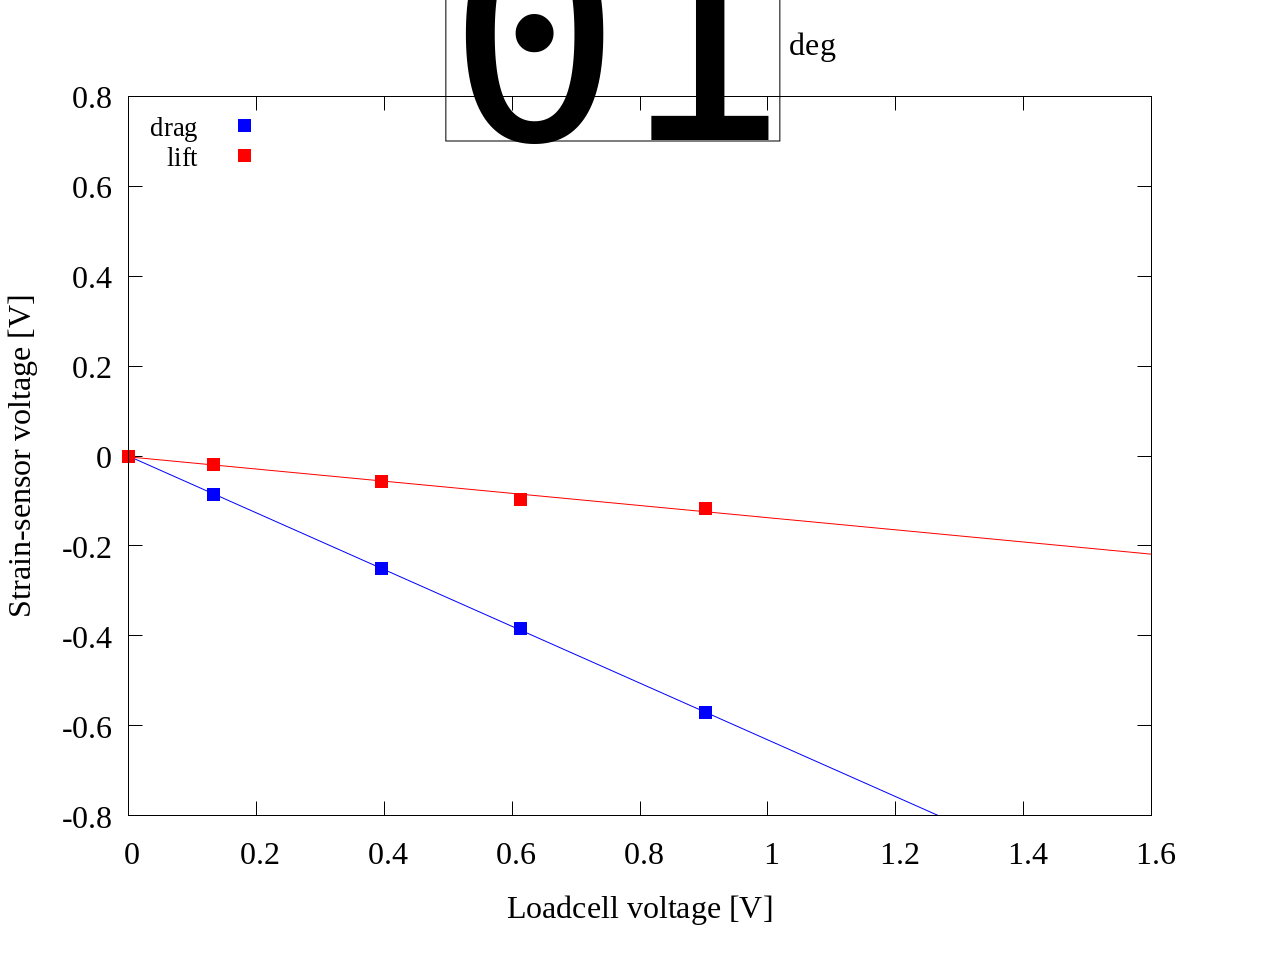
\includegraphics[width=80mm]{../images_2/04/04_linear_225.png}
        \caption{Correlation between loadcell and strainsensors 22.5 [deg]}
        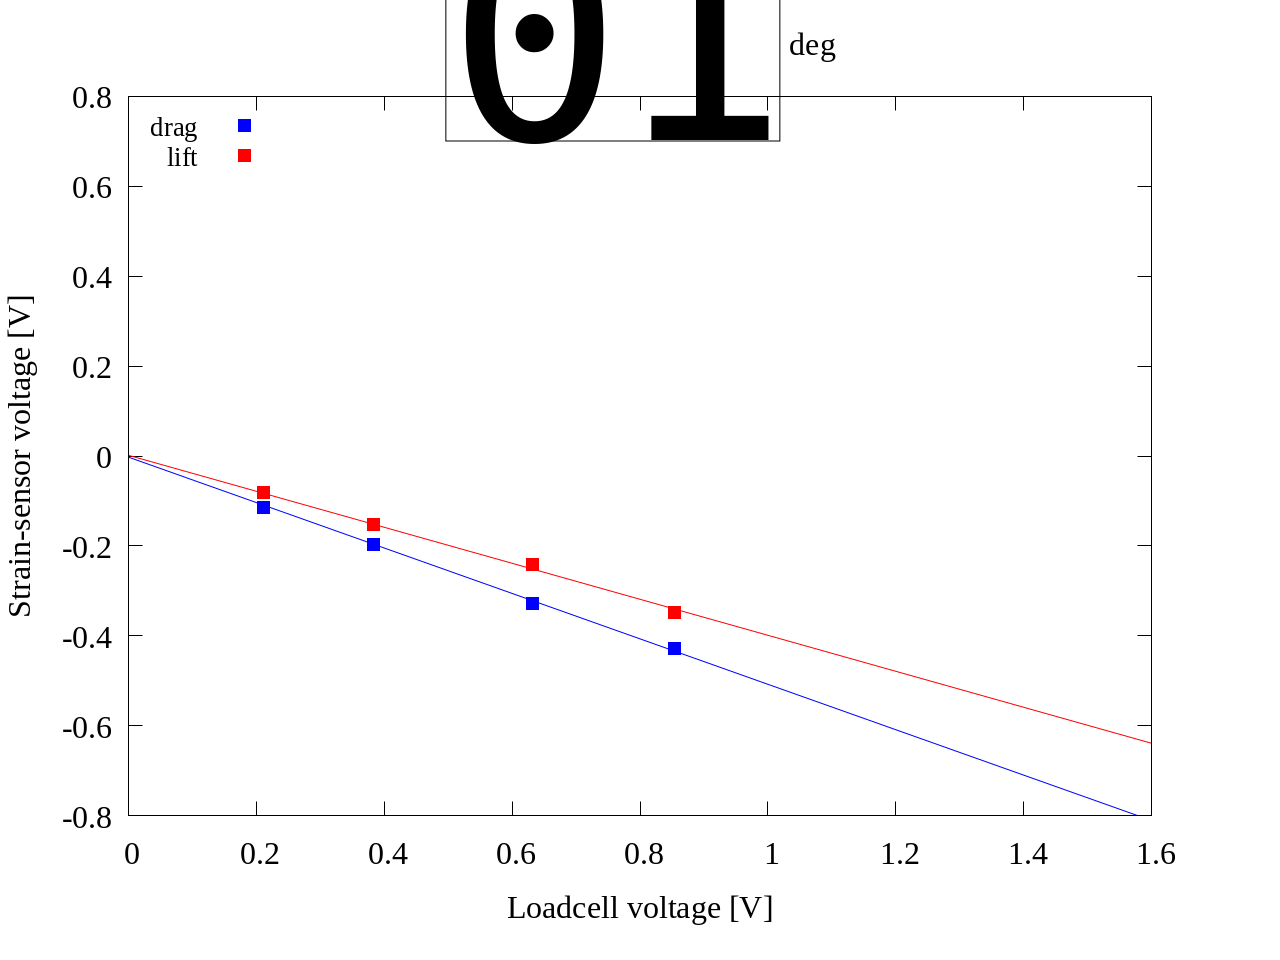
\includegraphics[width=80mm]{../images_2/04/04_linear_450.png}
        \caption{Correlation between loadcell and strainsensors 45.0 [deg]}
    \end{center}
\end{figure}

また,以下のFig.13に算出した近似直線の傾きについて角度ごとにプロットした図を示す.
\begin{itemize}
    \item [※] ここでの\textgt{"傾き"}とは,\textgt{"ロードセルの単位出力電圧あたりのひずみセンサの出力電圧"}を表している.
\end{itemize}

\begin{figure}[htbp]
    \footnotesize
    \begin{center}
        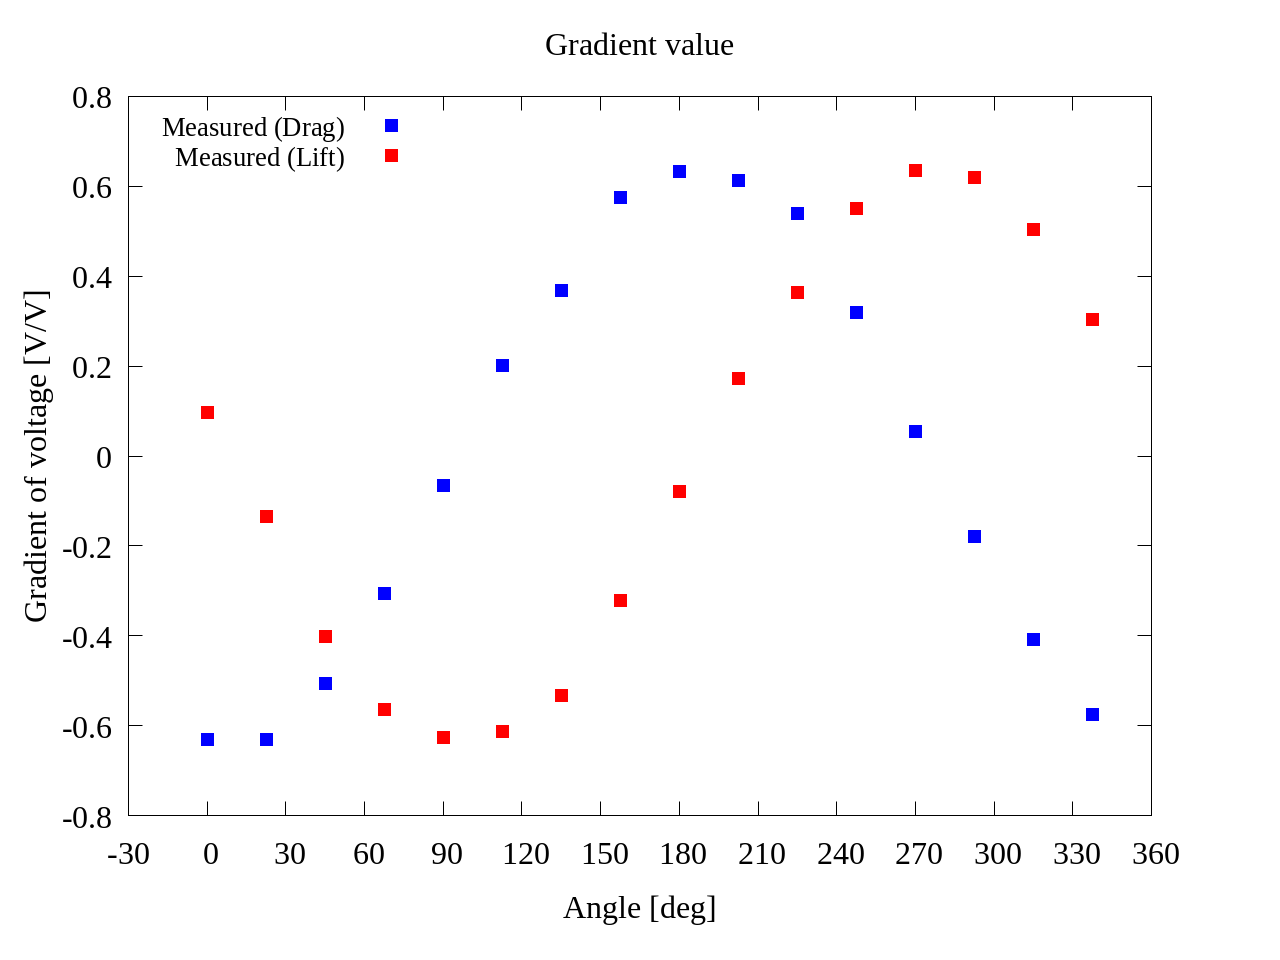
\includegraphics[width=92mm]{../images_2/05/05_summary-wave.png}
        \caption{Summary of gradient value}
    \end{center}
\end{figure}

\subsection{正味出力電圧の算出}
ここで,抗力・揚力方向のひずみセンサが直角に取り付けられていると仮定する.
このとき,抗力,揚力方向の傾きをそれぞれ$A_d$,$A_l$として,
以下の式に基づき正味出力電圧$A_{net}$を算出した.

\begin{itemize}
    \item [$\blacksquare$] \textgt{正味出力電圧の算出}
    \begin{eqnarray*}
        A_{net} = \sqrt{A_d^2 + A_l^2}\\
    \end{eqnarray*}
\end{itemize}

このときのそれぞれの角度における算出結果を以下のFig.14に示す.

\begin{figure}[htbp]
        \footnotesize
            \begin{center}
        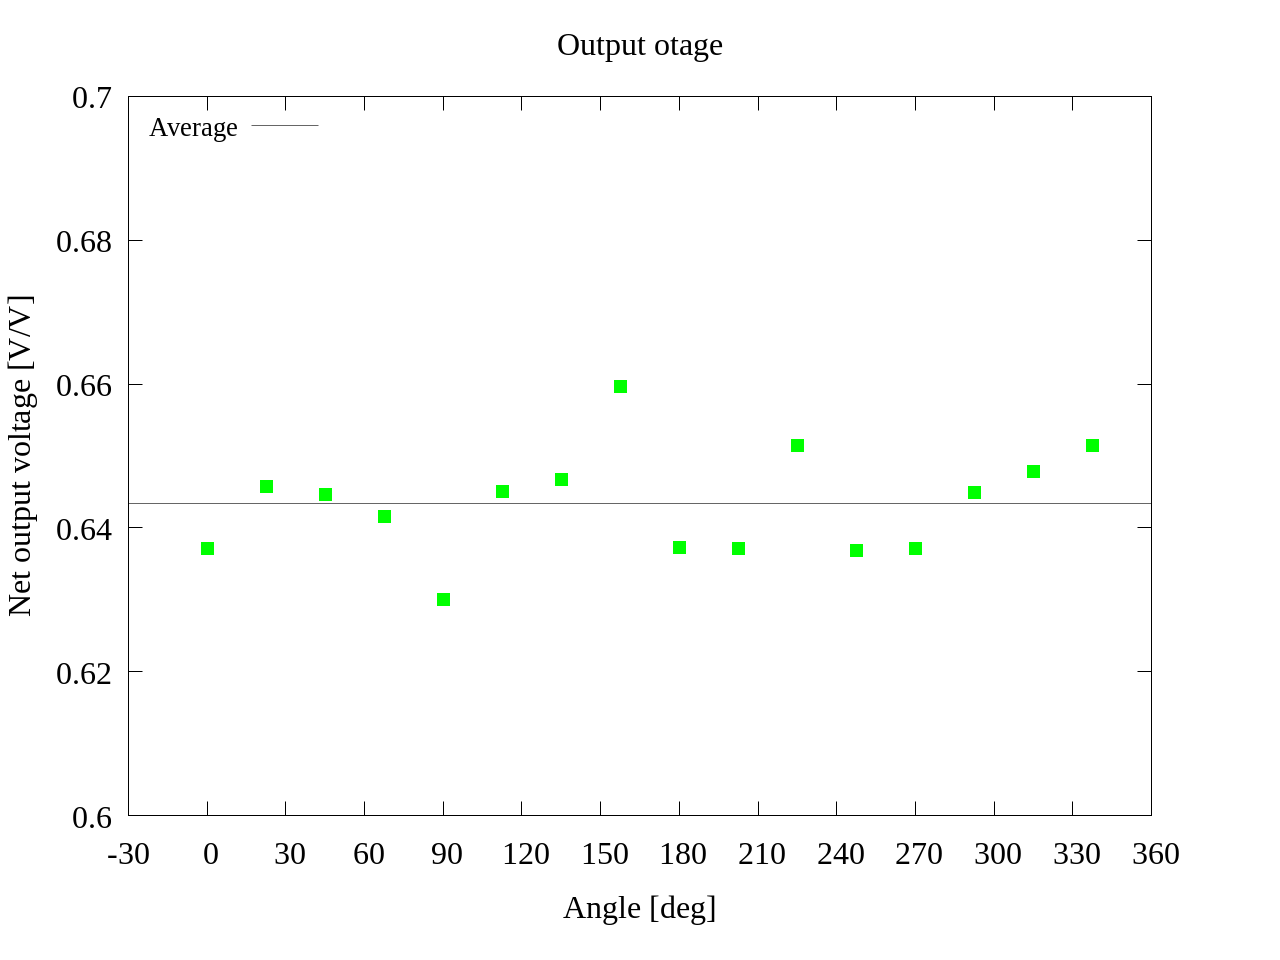
\includegraphics[width=92mm]{../images_2/05/05_summary-outputvoltage.png}
        \caption{Summary of net voltage value}
    \end{center}
\end{figure}

\newpage

また,それぞれの角度に対する傾きと正味出力電圧の値について
以下のTable.1に示す.

\begin{table}[htbp]
    \begin{center}
        \caption{Result summary}
        \begin{tabular}{|p{20mm}|p{20mm}|p{20mm}|p{20mm}|}
            \hline
            \multicolumn{1}{|c|}{\textgt{Angle [deg]}} & \multicolumn{1}{|c|}{\textgt{$A_d$ [V/V]}} & \multicolumn{1}{|c|}{\textgt{$A_l$ [V/V]}} & \multicolumn{1}{|c|}{\textgt{$A_{net}$ [V/V]}} \\ \hline
            \multicolumn{1}{|c|}{0.0}                  & \multicolumn{1}{|r|}{-0.630}           & \multicolumn{1}{|r|}{\textgt{0.096}}  & \multicolumn{1}{|r|}{\textgt{0.637}}  \\ \hline
            \multicolumn{1}{|c|}{22.5}                 & \multicolumn{1}{|r|}{-0.631}           & \multicolumn{1}{|r|}{\textgt{-0.135}}  & \multicolumn{1}{|r|}{\textgt{0.646}}  \\ \hline
            \multicolumn{1}{|c|}{45.0}                 & \multicolumn{1}{|r|}{-0.505}           & \multicolumn{1}{|r|}{\textgt{-0.400}}  & \multicolumn{1}{|r|}{\textgt{0.645}}  \\ \hline
            \multicolumn{1}{|c|}{67.5}                 & \multicolumn{1}{|r|}{-0.305}           & \multicolumn{1}{|r|}{\textgt{-0.564}}  & \multicolumn{1}{|r|}{\textgt{0.642}}  \\ \hline
            \multicolumn{1}{|c|}{90.0}                 & \multicolumn{1}{|r|}{-0.065}           & \multicolumn{1}{|r|}{\textgt{-0.627}}  & \multicolumn{1}{|r|}{\textgt{0.630}}  \\ \hline
            \multicolumn{1}{|c|}{112.5}                & \multicolumn{1}{|r|}{0.201}           & \multicolumn{1}{|r|}{\textgt{-0.613}}  & \multicolumn{1}{|r|}{\textgt{0.645}}  \\ \hline
            \multicolumn{1}{|c|}{135.0}                & \multicolumn{1}{|r|}{0.368}           & \multicolumn{1}{|r|}{\textgt{-0.532}}  & \multicolumn{1}{|r|}{\textgt{0.647}}  \\ \hline
            \multicolumn{1}{|c|}{157.5}                & \multicolumn{1}{|r|}{0.576}           & \multicolumn{1}{|r|}{\textgt{-0.322}}  & \multicolumn{1}{|r|}{\textgt{0.660}}  \\ \hline
            \multicolumn{1}{|c|}{180.0}                & \multicolumn{1}{|r|}{0.632}           & \multicolumn{1}{|r|}{\textgt{-0.079}}  & \multicolumn{1}{|r|}{\textgt{0.637}}  \\ \hline
            \multicolumn{1}{|c|}{202.5}                & \multicolumn{1}{|r|}{0.614}           & \multicolumn{1}{|r|}{\textgt{0.172}}  & \multicolumn{1}{|r|}{\textgt{0.637}}  \\ \hline
            \multicolumn{1}{|c|}{225.0}                & \multicolumn{1}{|r|}{0.540}           & \multicolumn{1}{|r|}{\textgt{0.365}}  & \multicolumn{1}{|r|}{\textgt{0.651}}  \\ \hline
            \multicolumn{1}{|c|}{247.5}                & \multicolumn{1}{|r|}{0.320}           & \multicolumn{1}{|r|}{\textgt{0.551}}  & \multicolumn{1}{|r|}{\textgt{0.637}}  \\ \hline
            \multicolumn{1}{|c|}{270.0}                & \multicolumn{1}{|r|}{0.054}           & \multicolumn{1}{|r|}{\textgt{0.635}}  & \multicolumn{1}{|r|}{\textgt{0.637}}  \\ \hline
            \multicolumn{1}{|c|}{292.5}                & \multicolumn{1}{|r|}{-0.180}           & \multicolumn{1}{|r|}{\textgt{0.619}}  & \multicolumn{1}{|r|}{\textgt{0.645}}  \\ \hline
            \multicolumn{1}{|c|}{315.0}                & \multicolumn{1}{|r|}{-0.407}           & \multicolumn{1}{|r|}{\textgt{0.504}}  & \multicolumn{1}{|r|}{\textgt{0.648}}  \\ \hline
            \multicolumn{1}{|c|}{337.5}                & \multicolumn{1}{|r|}{-0.576}           & \multicolumn{1}{|r|}{\textgt{0.305}}  & \multicolumn{1}{|r|}{\textgt{0.651}}  \\ \hline \hline
            \multicolumn{1}{|c|}{Average}              & \multicolumn{1}{|r|}{0.000}           & \multicolumn{1}{|r|}{\textgt{-0.002}}  & \multicolumn{1}{|r|}{\textgt{0.643}}  \\ \hline
        \end{tabular}
    \end{center}
\end{table}

また,正味出力電圧について算出した分散と標準偏差を以下のTable.2に示す.

\begin{table}[htbp]
    \begin{center}
        \caption{Net output voltage's variation and standard deviation}
        \begin{tabular}{|p{20mm}|p{20mm}|}
            \hline
            \multicolumn{1}{|c|}{\textgt{Variance}}     & \multicolumn{1}{|c|}{0.000051} \\ \hline
            \multicolumn{1}{|c|}{\textgt{Standard deviation}} & \multicolumn{1}{|c|}{0.007} \\ \hline
        \end{tabular}
    \end{center}
\end{table}

ここで,Table 1の正味出力電圧における平均値とTable 2の標準偏差を比較すると,
標準偏差は平均値の 1$\%$ 程度の範囲を示していることがわかる.

\begin{itemize}
    \item [$\blacksquare$] \textgt{平均値に対する標準偏差の割合}
    \begin{eqnarray*}
        \frac{0.007}{0.643} × 100 \approx 1.09 [\%]
    \end{eqnarray*}
\end{itemize}

したがって,標準偏差は平均値に対して十分小さい値であるといえ,
正味出力電圧は一定であると判断できると考えられる.

\newpage

\subsection{理論値の算出}
電圧の測定実験において,抗力および揚力の出力電圧は正弦波の位相がそれぞれ$-\pi/2$,$\pi$だけ
進んだ波形になると考えられる.
ここで,Table 1の正味出力電圧の平均値を振幅とし,
抗力および揚力についてそれぞれ位相が進んだ正弦波を作成した.
その算出結果と実験結果を重ねた図を以下のFig.15に示す.

\begin{itemize}
    \item [$\blacksquare$] \textgt{抗力・揚力における出力電圧の理論式}
    \begin{eqnarray*}
        V_{Drag} &=& A_{net} \sin\left(\omega t + \frac{3}{2}\pi\right) = A_{net} \cos\left(\omega t + \pi\right)\\
        V_{Lift} &=& A_{net} \sin\left(\omega t + \pi\right) = A_{net} \cos\left(\omega t + \frac{1}{2}\pi\right)
    \end{eqnarray*}
    \item [※] $A_{net}$はTable 2の正味出力電圧の平均値を使用
\end{itemize}

\begin{figure}[htbp]
    \footnotesize
    \begin{center}
        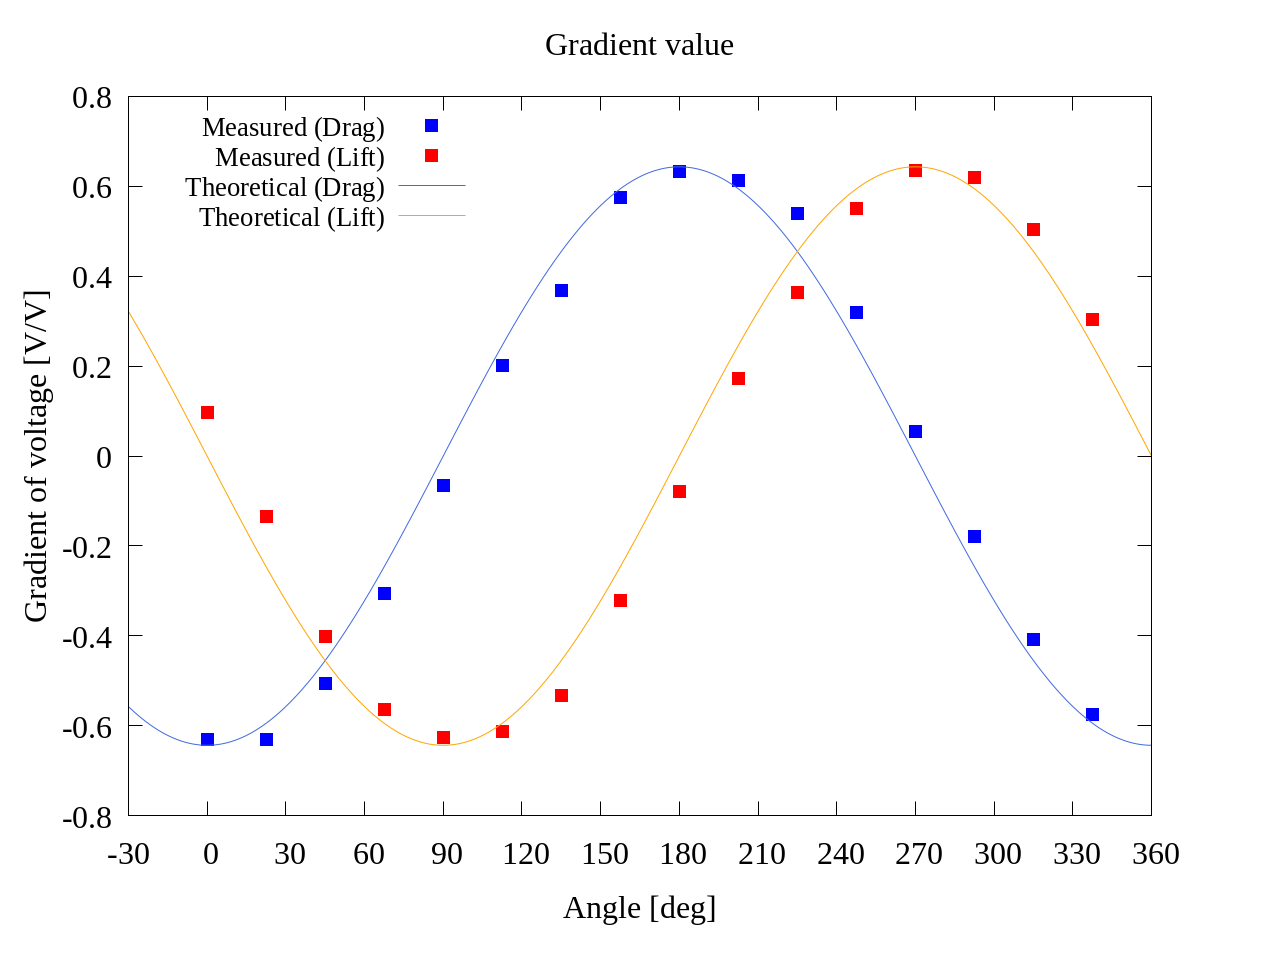
\includegraphics[width=92mm]{../images_2/20/20_adjust-value.png}
        \caption{theorical Value}
    \end{center}
\end{figure}

Fig.15をみると,実験結果は理論値に比べて抗力・揚力ともに位相が遅れていることがわかる.\\

\subsection{FFTの適用}
以上の結果から理論値との位相差を算出することを目的としてデータの処理を行う.
実験結果及び理論値についてFFTを適用した.その結果を以下のFig.16,Fig.17に,
波数1についての算出値をTable 3に示す.
\begin{table}[htbp]
    \begin{center}
        \caption{FFT result (Wave number [1])}
        \begin{tabular}{|p{20mm}|p{20mm}|p{20mm}|p{20mm}|}
            \hline
            \multicolumn{1}{|c|}{}                 & \multicolumn{1}{|c|}{\textgt{$Re$}} & \multicolumn{1}{|c|}{\textgt{$Im$}}       & \multicolumn{1}{|c|}{\textgt{Power}}     \\ \hline
            \multicolumn{1}{|c|}{Measured [Drag]}  & \multicolumn{1}{|r|}{-5.149}   & \multicolumn{1}{|r|}{\textgt{0.571}} & \multicolumn{1}{|r|}{\textgt{26.83}} \\ \hline
            \multicolumn{1}{|c|}{Measured [Lift]}  & \multicolumn{1}{|r|}{0.706}    & \multicolumn{1}{|r|}{\textgt{5.061}} & \multicolumn{1}{|r|}{\textgt{26.11}} \\ \hline
            \multicolumn{1}{|c|}{Theory [Drag]} & \multicolumn{1}{|r|}{-5.147}   & \multicolumn{1}{|r|}{\textgt{0.000}} & \multicolumn{1}{|r|}{\textgt{26.50}} \\ \hline
            \multicolumn{1}{|c|}{Theory [Lift]} & \multicolumn{1}{|r|}{0.000}    & \multicolumn{1}{|r|}{\textgt{5.147}} & \multicolumn{1}{|r|}{\textgt{26.50}} \\ \hline
        \end{tabular}
    \end{center}
\end{table}

\newpage

\begin{figure}[htbp]
    \footnotesize
    \begin{center}
        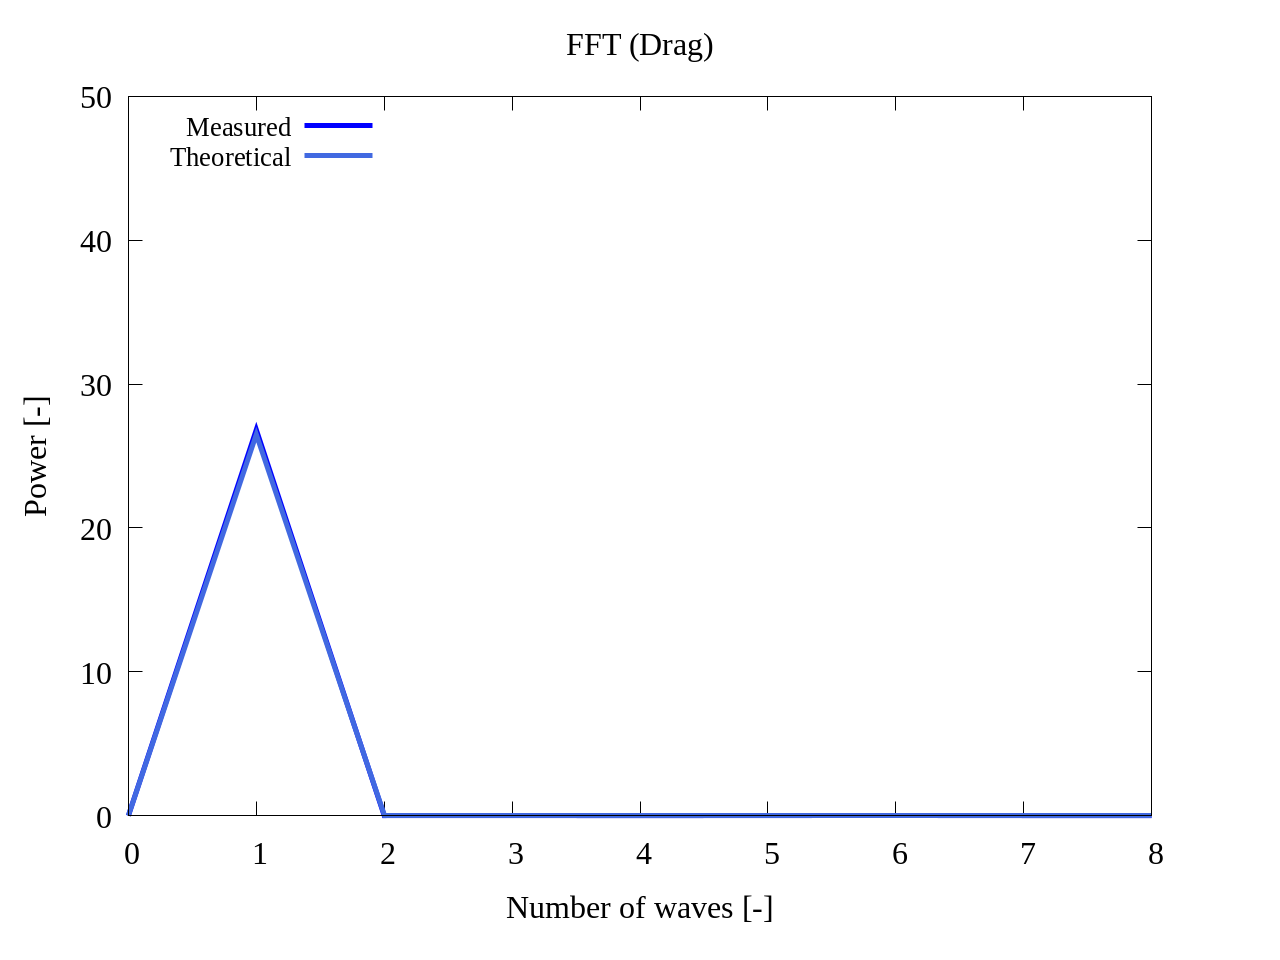
\includegraphics[width=83mm]{../images_2/27/27-3_fft-drag_summary.png}
        \caption{FFT Result (Drag)}
        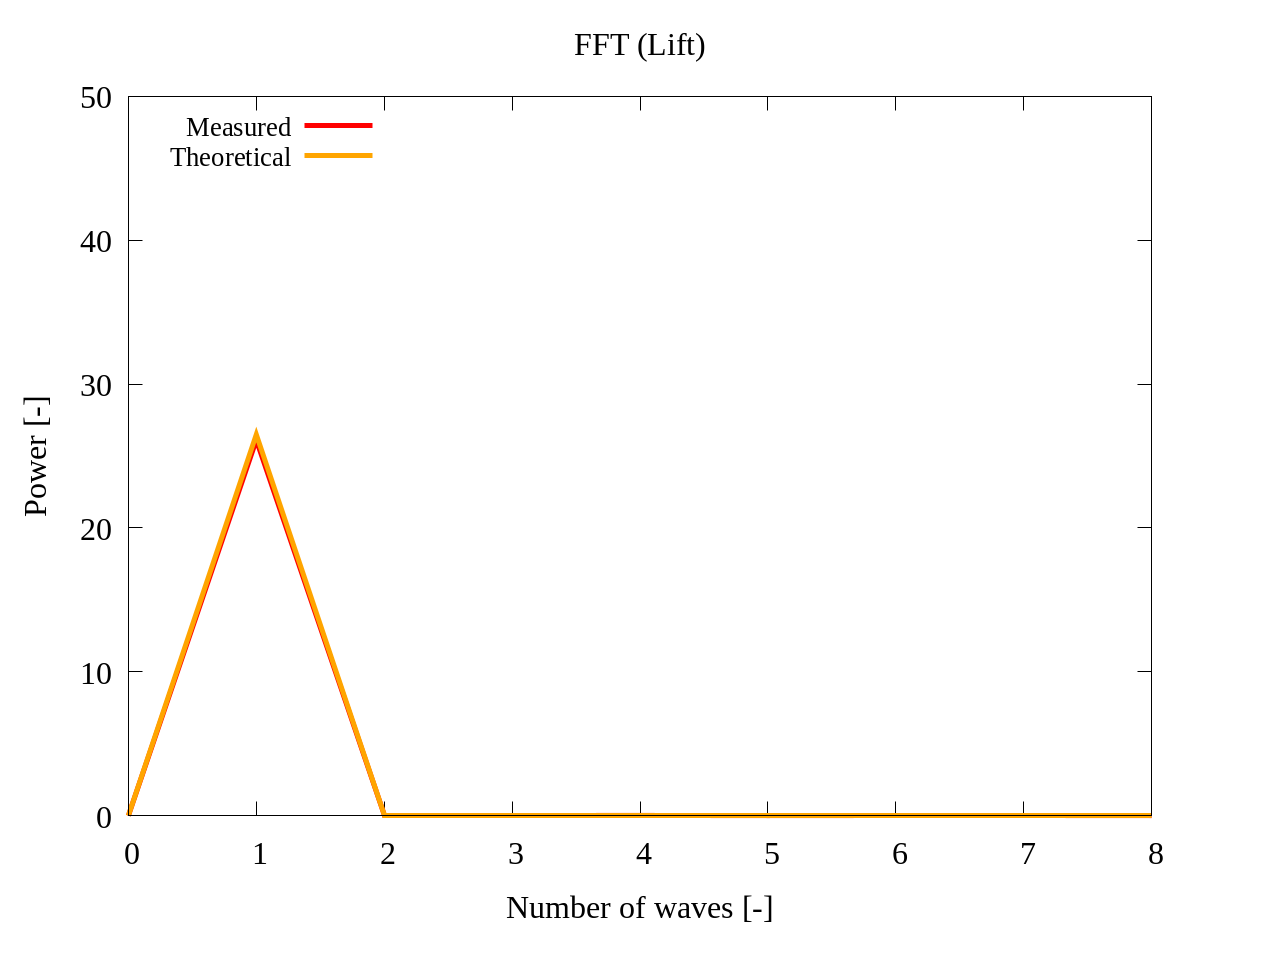
\includegraphics[width=83mm]{../images_2/27/27-4_fft-lift_summary.png}
        \caption{FFT Result (Lift)}
    \end{center}
\end{figure}

Fig.16,Fig.17をみると,実験結果と理論値のピークは一致していることがわかる.
また,Table 3をみると,パワースペクトル値は4つの条件に関しておおよそ一致していることがわかる.
したがって,FFTによって波の特徴を正しく捉えられており,抗力側及び揚力側に取り付けられているひずみセンサに
大きな個体差はないと考えられる.

\newpage

\subsection{理論値と実測値の位相角の算出}

ここで,Table 3の結果から以下の式をもとに位相角 $\phi$ を算出した.
抗力及び揚力方向の位相角をそれぞれ$\phi_x$,$\phi_y$として,その算出結果を以下のTable 4に示す.

\begin{itemize}
    \item [$\blacksquare$] 位相角$\phi$の算出
    \begin{eqnarray*}
        \mathrm{\phi \; [deg]} = \arctan \left(\frac{Im}{Re}\right) × \frac{180}{\pi}
    \end{eqnarray*}    
    \item [※] 位相角$\phi$は,FFTの性質上,余弦波に対する位相角を示している.
\end{itemize}

\begin{table}[htbp]
    \begin{center}
        \caption{Phase angle}
        \begin{tabular}{|p{20mm}|p{20mm}|p{20mm}|}
            \hline
            \multicolumn{1}{|c|}{}                    & \multicolumn{1}{|c|}{\textgt{$\phi_x$ [deg]}} & \multicolumn{1}{|c|}{\textgt{$\phi_y$ [deg]}} \\ \hline
            \multicolumn{1}{|c|}{\textgt{Measured}}   & \multicolumn{1}{|r|}{173.7}           & \multicolumn{1}{|r|}{82.1}           \\ \hline
            \multicolumn{1}{|c|}{\textgt{Theory}}  & \multicolumn{1}{|r|}{180.0}            & \multicolumn{1}{|r|}{90.0}           \\ \hline \hline
            \multicolumn{1}{|c|}{\textgt{Difference}} & \multicolumn{1}{|r|}{-6.3}           & \multicolumn{1}{|r|}{-7.9}           \\ \hline
        \end{tabular}
    \end{center}
\end{table}

Table 4をみると,実験で使用した回転台の回転座標を基準として,実験装置に取付けられたひずみセンサは
理論値に対して,抗力方向は -6.3 度,揚力方向は -7.9 度
進んでいることを示している.
したがって,回流水槽での作用力測定の際に,実際に加わる作用力の方向と
測定装置の設置角度に差異が存在している可能性があることがわかった.\\

\subsection{ひずみセンサの取付角の算出}

実験結果における抗力・揚力方向の位相角の差を取ることでひずみセンサの取付角度が算出できる.

\begin{itemize}
    \item [$\blacksquare$] 抗力・揚力方向のひずみセンサの取付角度 $\phi$
    \begin{eqnarray*}
        \phi &=& \left| \phi_x - \phi_y \right| \\
            &=& \left| 173.7 - 82.1 \right| \\
            &=& 91.6 \left[\mathrm{deg}\right]
    \end{eqnarray*}    
\end{itemize}

以上より,抗力・揚力方向のひずみセンサは 91.6 度の角度で取り付けられていることがわかった.
したがって,今回の実験装置について,ひずみセンサはおおよそ直角に貼付けられており,重大な課題ではないと考える.

\newpage

\section{今月のまとめと今後の予定}
\begin{itemize}
    \item [$\blacksquare$] 今月のまとめ
          \begin{itemize}
              \item [$\bullet$] 模擬実験を行い,今後の実験手順を検討・決定した
              \item [$\bullet$] 実験結果の処理プログラムを作成した
              \item [$\bullet$] 実験結果から,作用力と測定装置の設置角度を算出することができた
              \item [$\bullet$] 実験装置に取り付けられたひずみセンサの取付方向に大きな問題がないことが確認できた
          \end{itemize}
          \vskip\baselineskip
    \item [$\blacksquare$] 1月の予定
          \begin{itemize}
              \item [$\bullet$] 実験の実施 (1月末まで)
              \item [$\bullet$] 校正方法の検討
          \end{itemize}
\end{itemize}
\end{document}